\documentclass{beamer}
\usetheme[navigation]{UMONS}
\usepackage[utf8]{inputenc}
\usepackage[english]{babel}
\newcommand{\slideheight}{7.3cm}
\newcommand{\slidewidth}{12.3cm}

\title[Google File System]{The Google File System}
\author[B.Jason]{Jason \textsc{Bury}}
\institute[UMons-FS]{%
 Faculté des Sciences\\
  Université de Mons
  \\[2ex]
  
\includegraphics[height=4ex]{figures/UMONS}\hspace{2em}%
  \raisebox{-1ex}{
\includegraphics[height=6ex]{figures/UMONS_FS}}
}

% Le plan
% .Introduction
%   - Le problème
%   - Les observations, suppositions
%   - Les objectifs atteints
% .Architecture
%   - 1 maitres et des chunkservers
%   - Decoupage en chunk
%   - Ce que contient le maitre
% .Les garanties
% .Les interactions
%   - Lecture
%   - Les differentes etapes pour ecrire
%   - Append
%   - Snapshot
% .Master
%   - Namespace management (pas important)
%   - Replica placement
%   - Re-replication et rebalancing
% .Garbage collection
% .Mesures

\begin{document}
\maketitle

\section{Introduction}
\subsection{Introduction}
\newcommand{\incicon}[1]{\includegraphics[height=0.7cm]{figures/#1}}
% -The need of data processing is rapidly growing
% -There are thousands of inexpensive storage machine used by thousands of clients.
%  There is always one componenent failure and some will not recover.
% -The files are huge, typically multi-GB
% -The common files mutation here is data appending at the end of the file.
%  Writes withing a file are very rare.
\begin{frame} % TODO image de fond un big data floute grise
 \frametitle{The problems}
 \begin{itemize}
  \item \incicon{NPenhancement.png} Growing demands of data processing % icone augmente
  \item \incicon{NPbrokenDisc.png} Component failures % Icone casse
  \item \incicon{NPbigdataBlack.png} Huge files % Icone gros bloc de beton
  \item \incicon{NPpiled.png} Many appends % Icone pile
 \end{itemize}
\end{frame}

% -Many componenent that often fails
% -Few millions of files larger than 100MB and often Multi-GB. There can be also some small files.
% -Two kinds of reads: large streaming and small random reads
% -Writes are practically always large appends à the end of a file
% -Concurrent append to a file (Hundreds of producer and one consummer)
% -A high bandwith is far more appreciable than a low latency
\begin{frame}
 \frametitle{Assumptions}
 \begin{itemize}
  \item Many component that often fails
  \item Few millions of 100MB to Multi-GB files
  \item Large streaming reads
  \item Small random reads
  \item Large appends
  \item Rare random writes
  \item A high bandwith instead of low latency
 \end{itemize}
\end{frame}

% # ptet inutile
{
\usebackgroundtemplate{\vbox to \paperheight{\vfil\hbox to \paperwidth{\hfil
\includegraphics[height=7cm]{figures/CTR_Shield_3.jpg}\hfil}\vfil}}
\begin{frame}
 \frametitle{Guarantees}
 \begin{center}
 \begin{itemize}
  \item File namespace changements or creations are atomic. % By a lock
  \item All client will see the same. % Concurrent writing are made in the same order for each file and a number version for each chunk to detect stale chunk
 \end{itemize}
 \end{center}
\end{frame}
}

\section{Architecture}
\subsection{Architecture}
% # IMAGE avec master, des branches vers des cercles qui representent des clusters
% # Et dans ces clusters, mettre en etoiles des chunkservers avec ptet des pinguin linux
%
% The file system is distributed across multiple servers.
% All the files data are stored in chunkservers
% and a master server process all client's first request and maintain chunkservers to respect all guarantees.
\begin{frame}
 \frametitle{One Master, thousands chunkservers}
 \centering
 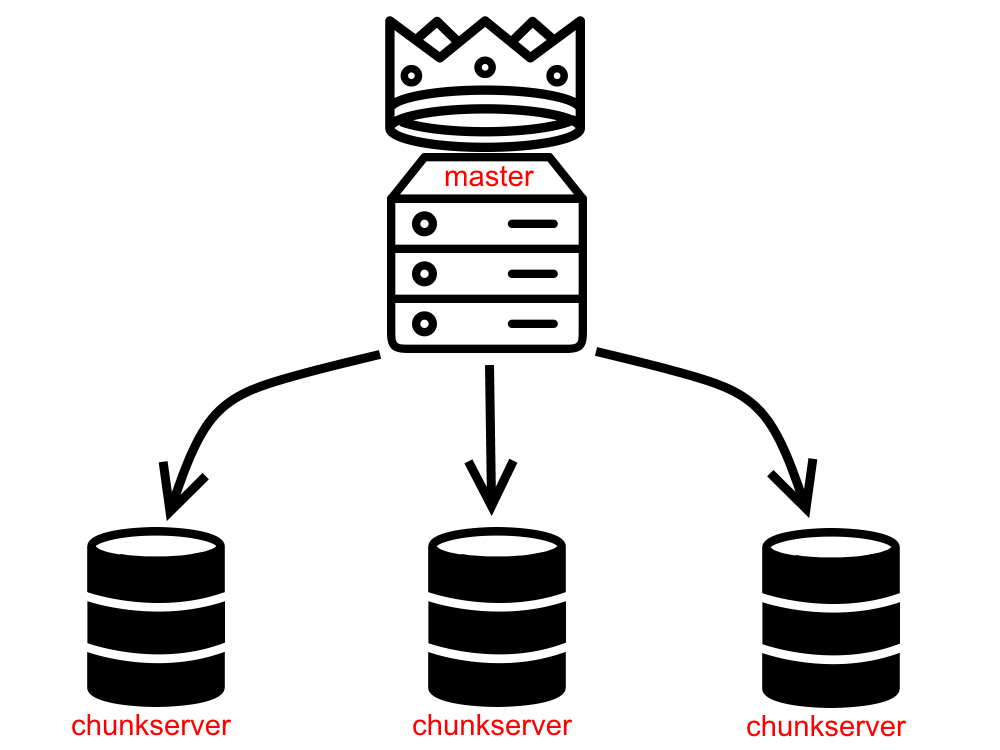
\includegraphics[height=\slideheight]{figures/masterschema.png}
\end{frame}

% # IMAGE voir derriere feuille. un fichier decoupe en chunks et 1 de ces chunks avec 3 fleches allant vers des chunkservers differentes
%
% Files are splitted into one ore several sixty-four Megabytes chunks.
% All chunks are replicated at least 3 times.
% The numbers of replica is chosen by the client.
% Then all replicas are stored in different chunkserver.
% and, more precisely, in different rack of chunkserver.
% So, the client lose access to its data only if all these chunkserver fails at the same time.
% and this case is unlikely from 3 replicas.
\begin{frame}
 \frametitle{A file}
 
\end{frame}

\newcommand{\masterpicheight}{5cm}
% # 1 IMAGE (ou 2) pour montrer l'arbre et le dictionnaire qu'il y a a coté.
%
% The master contains all metadatas about the file system.
% These metadatas are stored in three data structures.
% First, all file names are mapped to the list of unique IDs of their chunks. 
\begin{frame}
 \frametitle{The master}
 \framesubtitle{The file mapping}
 \centering
 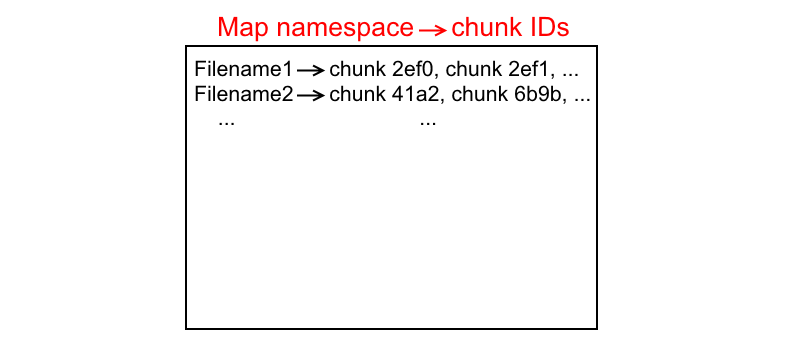
\includegraphics[height=\masterpicheight]{figures/namespaceMapschema.png}
\end{frame}
% Then, another mapping maps chunk IDs to the location of their replicas
\begin{frame}
 \frametitle{Master}
 \framesubtitle{The chunk mapping}
 \centering
 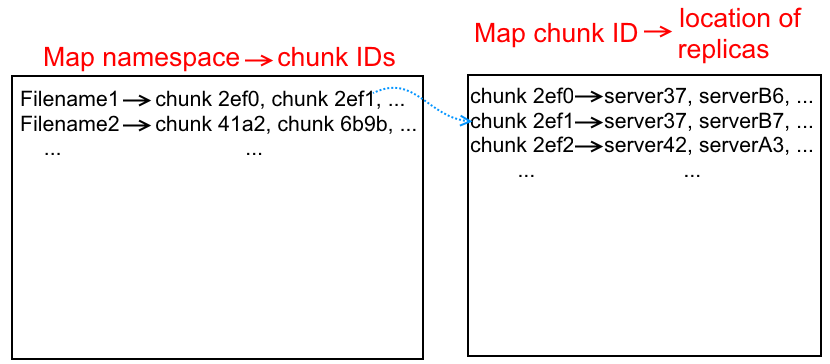
\includegraphics[height=\masterpicheight]{figures/namespaceMapMapschema.png}
\end{frame}
% And, To allow us to explore files like in i-node system,
% A tree organize the files and their name correspond to the namespace in the tree.TODO correct ?
\begin{frame}
 \frametitle{Master}
 \framesubtitle{The namespace tree}
 \centering
 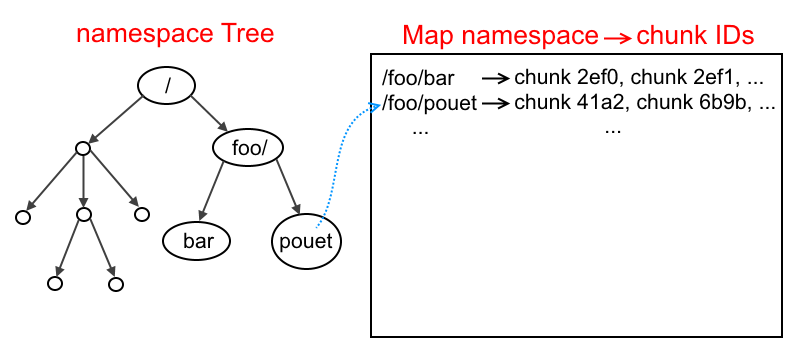
\includegraphics[height=\masterpicheight]{figures/namespaceTreeMapschema.png}
\end{frame}

\section{Interactions}
\subsection{Interactions}
% For a read,
% The client ask to the master, the location of a replica of a chunk providing the file name and the chunk index computed from chunk size and the offset.
% TODO Chunkserver state ?
% Then it responds with the chunk ID and the location of all replicas.
% No more interactions is needed between the client and the master.
% The client send its request to one of the chunkservers containing the desired replica.
% If the replica is not available, the client send the request again to another chunkserver containing the replica.
% And finally we have the data transfer.
\begin{frame}
 \frametitle{A read}
 \centering
 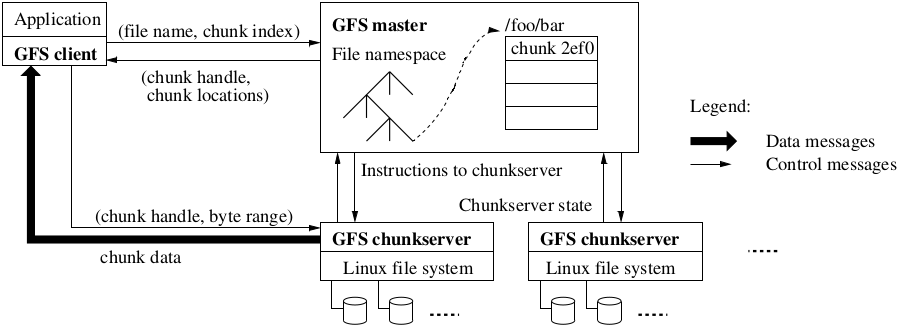
\includegraphics[width=\slidewidth]{figures/GFSarchitecture.png}
\end{frame}

% The write has to be made at all chunk replicas.
% First of all, the master grants one of the chunkservers containing a replica of the chunk to mutate.
% This chunkserver become the primary.
% So, step1, the client ask to the master which chunkserver is the primary and the location of chunk replicas.
% Step 2, the master respons and the client caches the primary identity
% so that, for future mutations to the chunk,
% no more interactions between the client and the master is needed until the primary become unreachable.
% Step 3, the data is transfered to the chunkservers.
% The maner that the data is transfered depends on the network topology and bandwith.
% Step 4, its time to write the data in the persistent memory:
% The client sends a write request to the primary.
% The primary can receive write request for the same chunk concurrently from different clients.
% It assign a serial number to all these request to define the order of mutation to do.
% Step 5, the primary sends the write request to secondary chunkservers providing the sequence of serial numbers.
% Then, step 6, all secondaries indicate to the primary that the operation is complete or failed.
% Finally, the primary indicates to the client if the write is a success or it failed in a secondary replica.
% If it failed, it loops starting at the thirs step were the client sends data to the secondary chunkserver that failed the operation.
% And if the fail still occur in some iterations of the loop, the client restart at step 1.
\begin{frame}
 \frametitle{A write}
 \centering
 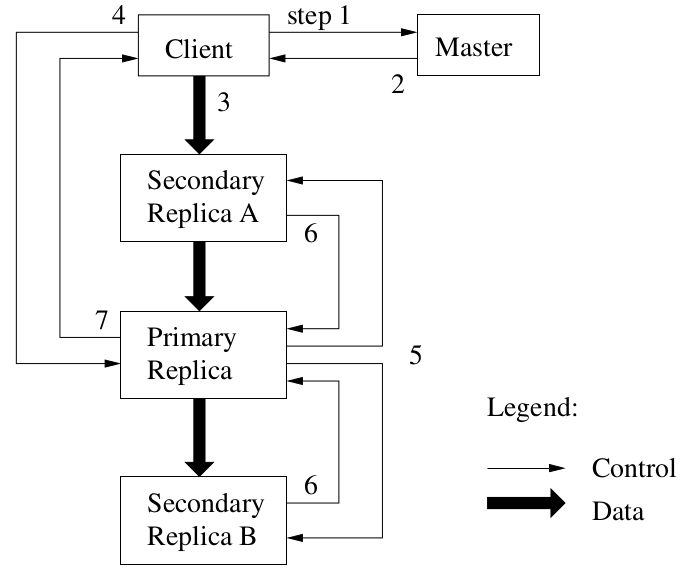
\includegraphics[height=\slideheight]{figures/GFSflow.png}
\end{frame}

% The random write in the same region can't be concurrent
% But if the write is an append, then the client doesn't have to inform the region where to write.
% The Google File System choose the offset where to write the append and this allow it to perform the write concurrently.
% The writing is performed as a multiple-producer/single-consumer queue.
\begin{frame}
 \frametitle{An append}
 
\end{frame}

\begin{frame}
 \frametitle{A snapshot}
 
\end{frame}

\section{Master's operations}
\subsection{Master operations}
\begin{frame}
 \frametitle{Replica placement}
 
\end{frame}

\begin{frame}
 \frametitle{Re-replica and rebalancing}
 
\end{frame}

\section{Rate measurements}
\subsection{Measurements}
\newcommand{\ratemesoption}{7cm}
\newcommand{\ratemehspace}{\hspace{15mm}}
\begin{frame}
 \frametitle{Read rate}
 \ratemehspace
 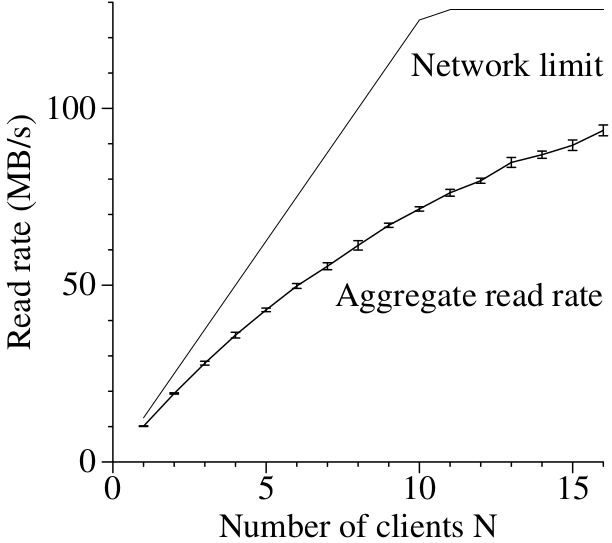
\includegraphics[height=\ratemesoption]{figures/GFSreads.png}
\end{frame}

\begin{frame}
 \frametitle{Write rate}
 \ratemehspace
 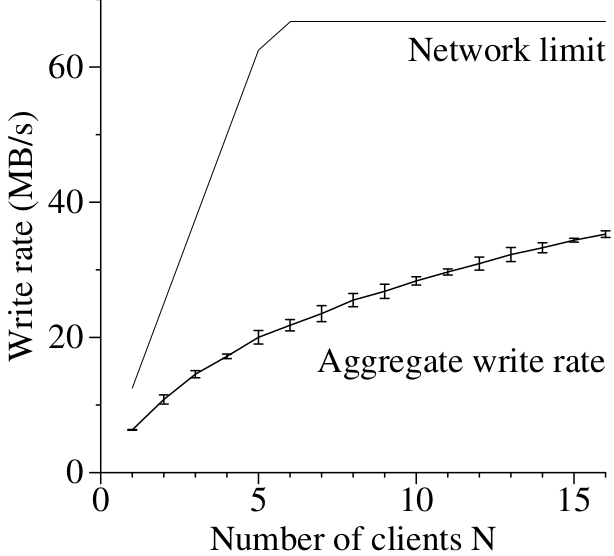
\includegraphics[height=\ratemesoption]{figures/GFSwrites.png}
\end{frame}

\begin{frame}
 \frametitle{Append rate}
 \ratemehspace
 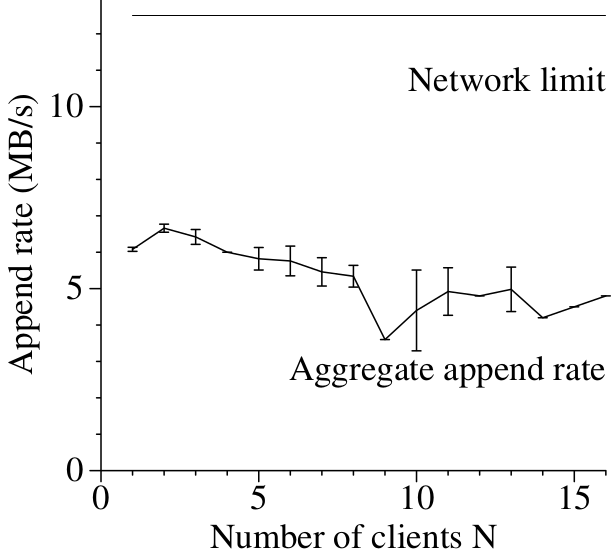
\includegraphics[height=\ratemesoption]{figures/GFSappends.png}
\end{frame}

\end{document}